% ==============================================================================
% Section 6: In-Silico Case Study (Central European Ecotone)
% ==============================================================================

\section{In-Silico Case Study: Central European Riparian-to-Floodplain-Meadow Ecotone}
\label{sec:case_studies}

To evaluate the coupled hybrid dynamical engine under multi-trophic heterogeneity, we construct and analyse a meso-scale \textbf{Central European Riparian-Woodland to Floodplain-Meadow Ecotone} on a $256 \times 256\,\text{m}$ ($6.55\,\text{ha}$, $1\,\text{m}^2$ per cell) periodic torus over a $4{,}000$-tick ($166.7$-day) temperate growing season. Four linked experiments examine the framework: (i) zero-shot spatial scale transfer ($128 \times 64 \to 256 \times 256$) and $10$-seed single-season community persistence, (ii) diagnostic evaluation of Propositions~\ref{thm:critical_synthesis_delay} and~\ref{thm:hopf_limit_cycle} under runtime kinetics, (iii) factorial wind and dual-channel ablation paired with a deterministic upwind relay experiment, and (iv) variance-based global sensitivity analysis with Common Random Numbers (CRN) across two spatial scales.

% ==============================================================================
\subsection{Ecological Context, Selection Rationale, and Biotope Construction}
\label{sec:ecotone_design}
% ==============================================================================

The modelled community represents lowland Central European river floodplains --- specifically the Oder and Elbe basins, including Brandenburg alluvial corridors --- where softwood riparian galleries (\textit{Salix}--\textit{Populus} stands and \textit{Ficario}--\textit{Ulmetum minoris} edges) grade into mesic floodplain grasslands (\textit{Arrhenatherion} meadows) and disturbed alluvial verges \cite{leuschner2017ecology, leuschner2017nonforest}. Prevailing summer airflow along WSW$\to$ENE ($22.5^\circ$) places the riparian fringe upwind on the western bank and the alluvial meadow downwind in the east. On the hourly lattice step, the wind vector $\mathbf{u}_{\text{wind}} = (0.878, 0.364)\,\text{cells/tick}$ ($\|\mathbf{u}_{\text{wind}}\| = 0.95\,\text{cells/tick}$) serves as the effective hourly plume-drift proxy defined in Section~\ref{subsec:atmospheric_transport} (scaling bounds are examined in Section~\ref{subsec:model_limitations}). Within $1\,\text{m}^2$ cells, woody taxa ($p_0, p_1$) represent juvenile floodplain saplings or clonal ramet patches whose reproduction intervals ($1{,}303\text{--}1{,}737\,\text{ticks}$) compress clonal recruitment into a single growing season, while herbivore guilds represent folivorous larval aggregations ($h_0, h_1, h_3, h_4$) and wingless aphid colonies ($h_2$) stepping at integer periods $v \in \{1, 2, 3\}\,\text{ticks/step}$.

Whereas simplified three-species orchard configurations omit growth--defence hierarchies, constitutive abrasion, inter-species root conduits, specialist counter-adaptations, and an embedded non-mycorrhizal control, the ecotone exercises every PHIDS mechanism inside its fixed 16-channel array layout ($6$ flora guilds, $5$ herbivore guilds, $9$ chemical channels $s_0$--$s_8$; Table~\ref{tab:case_study_configurations}). Six flora guilds span the growth--defence continuum: \textit{Populus nigra} ($p_0$, inducible green leaf volatile and terpenoid emitter with rapid vascular phloem withdrawal \cite{babst2005jasmonic, frost2008priming}); \textit{Salix purpurea} ($p_1$, high constitutive lignified and salicinoid armour \cite{boeckler2011phenolic, kayser2025pharmaceutical}); \textit{Trifolium repens} ($p_2$, high-degree arbuscular mycorrhizal hub with inducible cyanogenic glycosides and phloem withdrawal \cite{babikova2013underground, olsen2021dual, shen2023between, li2025common}); \textit{Lolium perenne} ($p_3$, constitutive silica phytoliths plus CMN-primed polyphenol oxidase escalation \cite{massey2006silica, shen2023between, li2025common}); \textit{Tanacetum vulgare} ($p_4$, aromatic ecotone fringe combining olfactory camouflage $\Phi_{\text{camo}}$ with proactive terpenoid deterrence \cite{clancy2016chemotypic}); and \textit{Brassica nigra} ($p_5$, non-mycorrhizal ruderal pioneer providing an embedded zero-CMN control \cite{schreiner1993stimulation, bekaert2012metabolic}).

Five herbivore guilds pair host specialisation with biochemical counter-adaptations: \textit{Lymantria dispar} ($h_0$, woody defoliator on $p_0, p_1$ \cite{lindroth2024forest}); \textit{Phratora vitellinae} ($h_1$, Salicaceae specialist tolerant of salicin \cite{pasteels1983salicin, kuhn2004selective}); \textit{Acyrthosiphon pisum} ($h_2$, phloem-feeding colony on $p_2$ \cite{shih2023pea}); \textit{Noctua pronuba} ($h_3$, polyphagous meadow generalist across $p_2$--$p_5$ \cite{topping2025noctua}); and \textit{Pieris brassicae} ($h_4$, crucifer specialist on $p_5$ whose nitrile-specifier proteins disarm allyl isothiocyanate escalation \cite{okamura2022testing}, realised in PHIDS by gating $s_7$ emission strictly to generalist $h_3$ feeding). Across the flora ($31$ trigger rules total), $10$ primary attack triggers initiate Stage-1 signalling, $3$ conditional rules govern phloem withdrawal on $p_0$--$p_2$, and $18$ conditionally gated rules coordinate secondary VOC relays and inducible toxins across riparian airborne priming ($s_0 \to s_1 \to s_3/s_4$), upwind meadow CMN relays ($s_2 \to s_6/s_8$), proactive $p_4$ deterrence ($s_5$), and generalist-gated $p_5$ escalation ($s_7$). All lethal toxins require composite priming-plus-grazing predicates, preventing unconditional firing on unattacked tiles.

Spatially, the ecotone is arranged across four overlapping habitat zones from west to east under the prevailing WSW$\to$ENE airflow (Table~\ref{tab:ecotone_spatial_init}, Fig.~\ref{fig:ecotone_spatial_snapshot}a). Thomas cluster processes establish upwind riparian galleries of \textit{Populus nigra} and \textit{Salix purpurea} across the western terrace and downwind meadow stands of \textit{Trifolium repens} and \textit{Lolium perenne} across the eastern floodplain. Between them, a bimodal inhomogeneous Poisson intensity creates an aromatic transition fringe of \textit{Tanacetum vulgare} centred near the woodland margin ($x = 112$) and the western edge ($x = 16$). Finally, thinned circular micro-patches of \textit{Brassica nigra} occupy alluvial gaps and woodland clearings under checkerboard parity and strict cardinal-neighbour exclusion, enforcing zero mycorrhizal connectivity ($\overline{\deg}_{\text{CMN}}(p_5) = 0.00$) alongside $61.9\%$--$85.4\%$ initial connectivity across $p_0$--$p_4$. Initialisation places $14{,}679$ plants ($22.40\%$ cover) and $72$ founder swarms ($1{,}554$ individuals) on the $256 \times 256$ flagship lattice, and $1{,}941$ plants ($23.69\%$ cover) with $20$ founder swarms ($208$ individuals) on the $128 \times 64$ calibration twin. Figure~\ref{fig:ecotone_spatial_snapshot} shows a live state snapshot at tick $331$ together with a $56 \times 56$ transition detail resolving individual cardinal root links, herbivore swarms, and downwind VOC plumes.

\begin{figure*}[t]
  \centering
  % ==============================================================================
% Figure 6 (LaTeX fig08): Spatial Ecotone Snapshot & Zoomed Transition ROI
% ==============================================================================

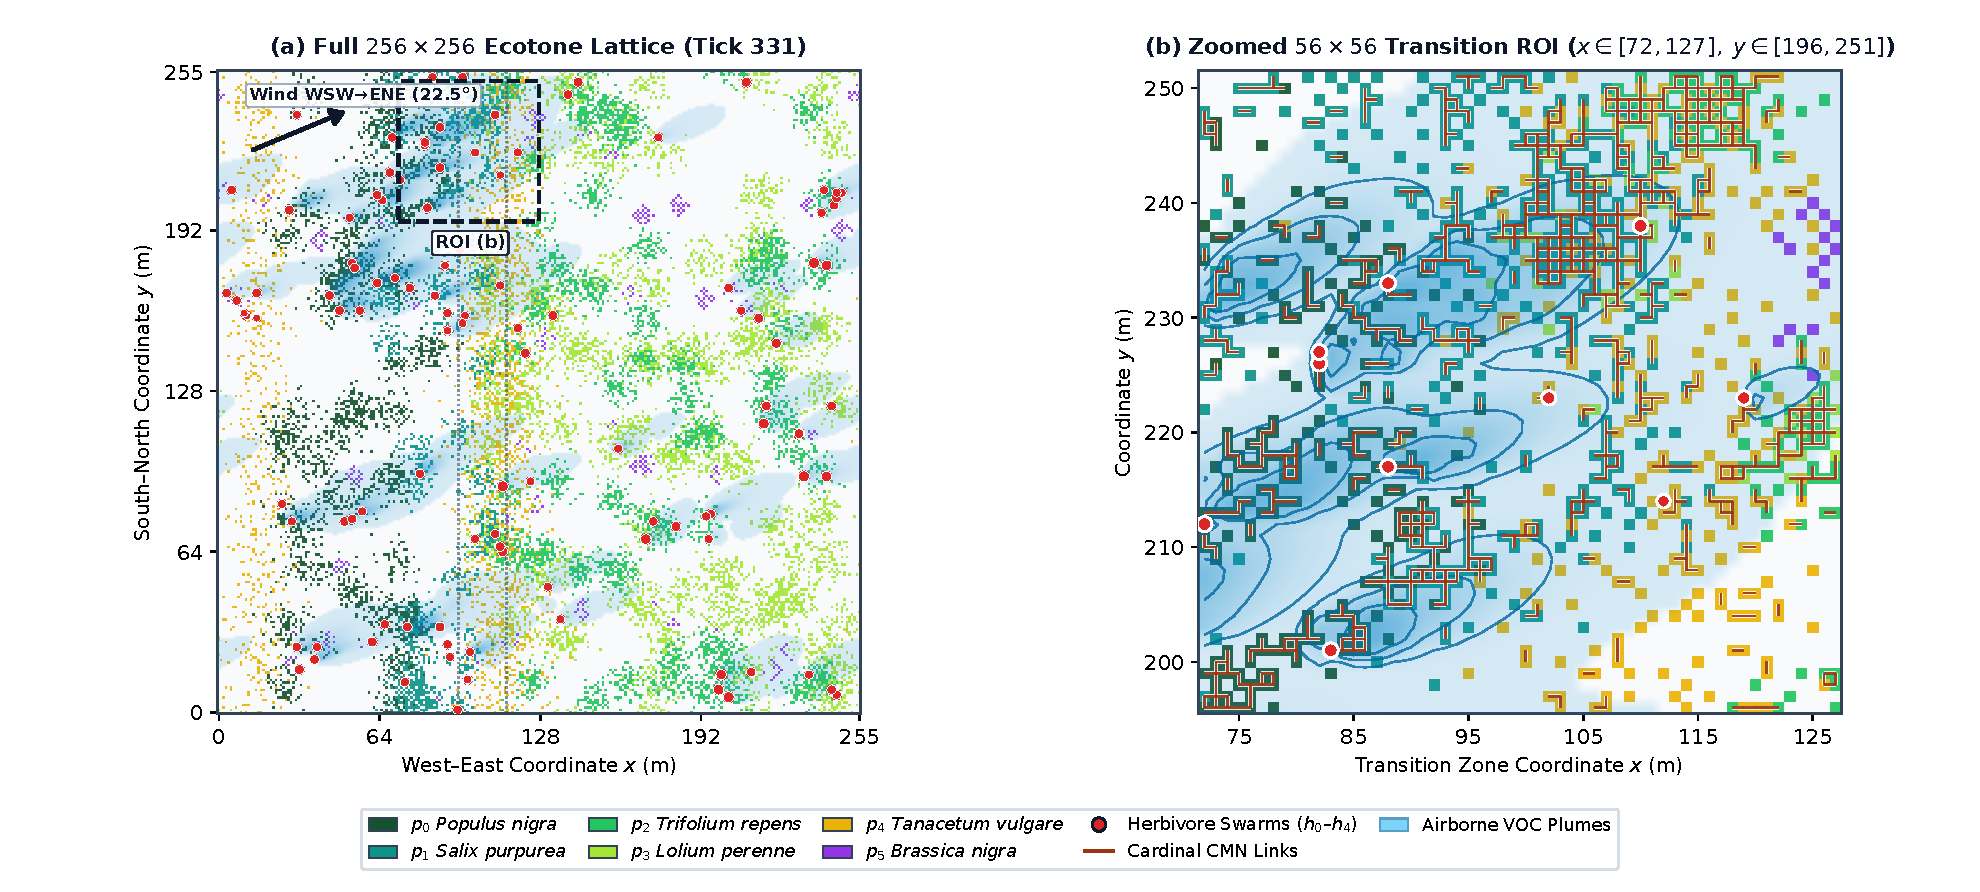
\includegraphics[width=\textwidth]{figures/fig08_ecotone_spatial_snapshot.pdf}

  \caption{Spatial State Snapshot of the Calibrated $256 \times 256$ Central European Ecotone at Tick $331$ ($13{,}880$ active plants, $128$ herbivore swarms comprising $3{,}867$ individuals, and $10{,}331$ undirected cardinal mycorrhizal links). \textbf{(a)} Full $256 \times 256\,\mathrm{m}$ lattice showing upwind western riparian woodland ($p_0, p_1$), the aromatic \textit{Tanacetum} transition fringe ($p_4$), the downwind eastern meadow ($p_2, p_3$), isolated non-mycorrhizal \textit{Brassica nigra} patches ($p_5$), airborne VOC plumes ($C_{s_0\text{--}s_2}$), and herbivore swarms under WSW$\to$ENE ($22.5^\circ$) plume drift. \textbf{(b)} Zoomed $56 \times 56$ transition window ($x \in [72, 128)$, $y \in [196, 252)$; $1{,}020$ plants, $11$ swarms, $868$ interior cardinal root links) resolving cell-level guild boundaries, explicit mycorrhizal edges, and local VOC dispersion contours.}
  \label{fig:ecotone_spatial_snapshot}
\end{figure*}

\begin{table*}[b]
\caption{Spatial Point-Process Initialisation Parameters and Initial Cardinal Mycorrhizal Connectivity on the $256 \times 256$ Ecotone.}
\label{tab:ecotone_spatial_init}
\vspace{4pt}
\centering
\scriptsize
\setlength{\tabcolsep}{2.5pt}
\begin{tabularx}{\textwidth}{
  >{\raggedright\hsize=1.08\hsize}X
  >{\raggedright\hsize=0.90\hsize}X
  >{\centering\hsize=0.82\hsize}X
  >{\centering\hsize=0.80\hsize}X
  >{\raggedright\hsize=1.10\hsize}X
  >{\raggedright\hsize=1.10\hsize}X
  >{\raggedright\arraybackslash\hsize=1.20\hsize}X
}
\toprule
\textbf{Flora Guild} & \textbf{Spatial Process} & \textbf{Domain Band ($x$)} & \textbf{Parents / Patches} & \textbf{Intensity / Offspring} & \textbf{Dispersion / Exclusion} & \textbf{Initial $N_0$ / CMN Conn.} \\
\midrule
$p_0$ \textit{Populus nigra}     & Thomas cluster & $x \in [22, 88]$   & $55$ parents & $\mathrm{Poisson}(65)$ & $\sigma_r = 4.2\,\mathrm{m}$ & $2{,}755$ ($78.3\%$, $\overline{\deg}=1.59$) \\
$p_1$ \textit{Salix purpurea}    & Thomas cluster & $x \in [66, 110]$  & $42$ parents & $\mathrm{Poisson}(55)$ & $\sigma_r = 3.8\,\mathrm{m}$ & $1{,}698$ ($85.0\%$, $\overline{\deg}=1.87$) \\
$p_2$ \textit{Trifolium repens}  & Thomas cluster & $x \in [114, 244]$ & $65$ parents & $\mathrm{Poisson}(75)$ & $\sigma_r = 3.6\,\mathrm{m}$ & $3{,}552$ ($85.4\%$, $\overline{\deg}=1.88$) \\
$p_3$ \textit{Lolium perenne}    & Thomas cluster & $x \in [106, 248]$ & $85$ parents & $\mathrm{Poisson}(70)$ & $\sigma_r = 4.5\,\mathrm{m}$ & $4{,}346$ ($76.6\%$, $\overline{\deg}=1.48$) \\
$p_4$ \textit{Tanacetum vulgare} & Bimodal inh.\ Poisson & Peaks $x = 112, 16$ & $2$ Gaussian bands & $p_{\max} = 0.24, 0.14$ (cap $0.35$) & $\sigma = 9, 7\,\mathrm{m}$ & $1{,}871$ ($61.9\%$, $\overline{\deg}=1.11$) \\
$p_5$ \textit{Brassica nigra}    & Thinned micro-patches & $48$ gap / $12$ core & $60$ discs ($r = 4$) & Checkerboard ($p = 0.72$) & Zero cardinal neighbours & $457$ ($0.0\%$, $\overline{\deg}=0.00$) \\
\bottomrule
\multicolumn{7}{@{}p{\textwidth}@{}}{Flagship $256 \times 256$ initialisation yields $14{,}679$ plants ($22.40\%$ cover) and $72$ founder swarms ($1{,}554$ individuals). The $128 \times 64$ reduced-lattice calibration twin scales parent and patch counts proportionally to lattice area ($1{,}941$ plants, $23.69\%$ cover, $20$ founder swarms comprising $208$ individuals).}
\end{tabularx}
\end{table*}

% ==============================================================================
% Table 4 (LaTeX tab07): Calibrated Central European Ecotone Parameterisation
% Placed at bottom [b] of page, caption above table
% ==============================================================================

\begin{table*}[b]
\caption{Calibrated Parameterisation of the Central European Riparian-to-Floodplain-Meadow Ecotone ($256 \times 256$ Flagship and $128 \times 64$ Reduced-Lattice Twin).}
\label{tab:case_study_configurations}
\vspace{4pt}
\centering
\scriptsize
\setlength{\tabcolsep}{1.6pt}
\begin{tabular*}{\textwidth}{@{\extracolsep{\fill}} l c c c c c c c c @{}}
\toprule
\multicolumn{9}{@{}l}{\textbf{Panel A: Six Sympatric Flora Guilds ($p_0$--$p_5$)} --- Cohort growth $r_p$, seed dist.\ $[d_{\min},d_{\max}]$ ($p_0{:}6\text{--}28$, $p_1{:}5\text{--}22$, $p_2{:}1\text{--}5$, $p_3{:}1\text{--}8$, $p_4{:}1\text{--}6$, $p_5{:}1\text{--}4$)} \\
\midrule
\textbf{Flora Species} &
\textbf{$E_{\mathrm{b}}/E_{\max}/E_{\min}$} &
\textbf{$r_p$} &
\textbf{Repro / $E_{\text{seed}}$} &
\textbf{$c_{\text{bite}}$ / $(1{-}\delta_m)$} &
\textbf{$\Phi_{\text{camo}}$} &
\textbf{$\eta_{\min}$ / $\gamma_{\text{tr}}$} &
\textbf{$\delta_E^{\text{tax}}$} &
\textbf{$N_0$ / $\overline{\deg}_{\text{CMN}}$} \\
\midrule
$p_0$ \textit{Populus nigra}     & $70/140/14$ & $0.1500$ & $1303$ / $56.00$ & $0.05$ / $0.88$ & $1.00$ & $0.45$ / $0.08$ & $0.65$ & $2{,}755$ / $1.59$ \\
$p_1$ \textit{Salix purpurea}    & $60/120/12$ & $0.0935$ & $1737$ / $48.00$ & $0.15$ / $0.62$ & $1.00$ & $0.70$ / $0.05$ & $0.55$ & $1{,}698$ / $1.87$ \\
$p_2$ \textit{Trifolium repens}  & $45/85/9$   & $0.3000$ & $1086$ / $34.15$ & $0.00$ / $0.96$ & $1.00$ & $0.55$ / $0.10$ & $0.50$ & $3{,}552$ / $1.88$ \\
$p_3$ \textit{Lolium perenne}    & $55/105/11$ & $0.3200$ & $1086$ / $42.69$ & $0.22$ / $0.68$ & $1.00$ & $---$ / $0.06$  & $0.50$ & $4{,}346$ / $1.48$ \\
$p_4$ \textit{Tanacetum vulgare} & $50/100/10$ & $0.1800$ & $1737$ / $40.00$ & $0.04$ / $0.86$ & $0.35$ & $---$ / $0.05$  & $0.35$ & $1{,}871$ / $1.11$ \\
$p_5$ \textit{Brassica nigra}    & $35/68/7$   & $0.5200$ & $868$ / $24.40$  & $0.00$ / $0.97$ & $1.00$ & $---$ / $0.05$  & $0.00$ & $457$ / $0.00$ \\
\bottomrule
\end{tabular*}

\vspace{3pt}
\begin{tabular*}{\textwidth}{@{\extracolsep{\fill}} l c c c c c c c c @{}}
\toprule
\multicolumn{9}{@{}l}{\textbf{Panel B: Five Herbivore Guilds ($h_0$--$h_4$) \& Diet Matrix $\mathbf{D}$} --- Per-stride $a$ ($\mathrm{stride}^{-1}$), $T_h^{\mathrm{stride}}$ ($\mathrm{stride}\cdot\mathrm{cal}^{-1}$), $\Delta_{\mathrm{stride}}{=}1.0$; hourly $U$} \\
\midrule
\textbf{Herbivore Guild} &
\textbf{Diet Hosts} &
\textbf{$v$} &
\textbf{$a$} &
\textbf{$T_h^{\mathrm{stride}}$} &
\textbf{$E_{\min}$ / $U$} &
\textbf{Div. / Split} &
\textbf{$(\alpha_m, \alpha_c, e_{\text{eff}})$} &
\textbf{Swarms} \\
\midrule
$h_0$ \textit{Lymantria dispar}   & $\{p_0, p_1\}$         & $2$ & $3.3337$ & $0.1140$ & $1.40$ / $.00843$ & $2.1$ / $26$ & $(.10, .05, .38)$ & $14{\times}18$ / $4{\times}9$ \\
$h_1$ \textit{Phratora vitellinae}& $\{p_0, p_1\}$         & $2$ & $2.3523$ & $0.1726$ & $1.00$ / $.00991$ & $2.5$ / $24$ & $(.35, .20, .42)$ & $12{\times}16$ / $4{\times}8$ \\
$h_2$ \textit{Acyrthosiphon pisum}& $\{p_2\}$              & $1$ & $2.6664$ & $0.1268$ & $1.10$ / $.01215$ & $2.0$ / $46$ & $(.15, .05, .65)$ & $18{\times}35$ / $4{\times}18$ \\
$h_3$ \textit{Noctua pronuba}     & $\{p_2..p_5\}$         & $3$ & $1.5139$ & $0.3342$ & $1.10$ / $.01055$ & $2.4$ / $26$ & $(.15, .10, .48)$ & $16{\times}18$ / $4{\times}9$ \\
$h_4$ \textit{Pieris brassicae}   & $\{p_5\}$              & $2$ & $2.7064$ & $0.1633$ & $1.00$ / $.00981$ & $2.4$ / $24$ & $(.20, .15, .44)$ & $12{\times}16$ / $4{\times}8$ \\
\bottomrule
\end{tabular*}

\vspace{3pt}
\begin{tabular*}{\textwidth}{@{\extracolsep{\fill}} l l c c c c c l @{}}
\toprule
\multicolumn{8}{@{}l}{\textbf{Panel C: Chemical Channels ($s_0$--$s_8$) \& $31$-Rule Cascade} --- $\mathbf{u}=(0.878,0.364)\,\mathrm{cells/tick}$, decay $0.82$, emit $0.55$, $c_{\mathrm{conn}}=0.5$, $g_{\mathrm{relay}}=2$} \\
\midrule
\textbf{ID} &
\textbf{Compound \& Functional Class} &
\textbf{Sources} &
\textbf{Hill / Lethal} &
\textbf{Walk} &
\textbf{$\theta_{\text{p}}/\theta_{\text{u}}$} &
\textbf{Aft.} &
\textbf{Trigger Gating Summary} \\
\midrule
$s_0$ & (Z)-3-Hexenyl Acetate (GLV signal)      & $p_0,p_1,p_4,p_5$ & $K_d{=}0.133, n{=}3$ & $---$ & $---/1$ & $6$  & Stage-1 attack ($p_0,p_1,p_4,p_5$) \\
$s_1$ & (E)-$\beta$-Ocimene / DMNT (relay)      & $p_0,p_1$         & $K_d{=}0.093, n{=}3$ & $---$ & $1/---$ & $8$  & Gated on $C_{s_0}\ge 0.05$ \\
$s_2$ & MeSA + CMN Jasmonate (VOC/hyphal)       & $p_0,p_1,p_2,p_3$ & $K_d{=}0.109, n{=}2$ & $---$ & $---/3$ & $12$ & Stage-1 attack ($p_0,p_1,p_2,p_3$) \\
$s_3$ & Benzyl Cyanide (repellent toxin)        & $p_0$             & $c_{\text{synth}}{=}0.11$ & $5$ & $2/12$ & $14$ & $s_0$ active or $h_0$/$s_1$ primed \\
$s_4$ & Kunitz TI / Salicinoids (lethal toxin)  & $p_0,p_1$         & $0.0625$ / $0.0547$  & $---$ & $2/12$  & $18$ & Composite conjunctive/disjunctive gates \\
$s_5$ & $\beta$-Thujone / Camphor (repellent)   & $p_4$             & $c_{\text{synth}}{=}0.10$ & $8$ & $1/3$  & $16$ & $s_0$/$s_2$ curtain or $h_3$ + $s_0$ \\
$s_6$ & \textit{Trifolium} HCN (lethal+repel.)  & $p_2$             & $0.0839$             & $5$   & $1/8$   & $12$ & $s_2$ + $h_3$ primed/attack gate \\
$s_7$ & Allyl Isothiocyanate (lethal AITC)      & $p_5$             & $0.0671$             & $---$ & $2/8$   & $16$ & Gated solely to generalist $h_3$ \\
$s_8$ & \textit{Lolium} PPO + Silica (lethal)   & $p_3$             & $0.0923$             & $---$ & $2/10$  & $16$ & $s_2$ + $h_3$ primed/attack gate \\
\bottomrule
\end{tabular*}
\par\vspace{2pt}
\raggedright\scriptsize\textit{Note:} Woody taxa ($p_0,p_1$) represent juvenile floodplain saplings/clonal ramets ($1\,\mathrm{m}^2$ cells; $g_{\mathrm{struct}} \in \{0.008, 0.010, 0.006, 0.008, 0.007, 0.005\}$ with $M_{\max}=E_{\max}$). Herbivore integer period $v$ gives step cadence $1/v \in \{0.33, 0.50, 1.00\}\,\mathrm{cells/h}$; feeding parameters $a$ and $T_h^{\mathrm{stride}}$ govern each diurnal feeding stride ($\Delta_{\mathrm{stride}} = 1.0$, Eq.~\eqref{eq:math_holling_type_ii}). Setting $E_{\mathrm{base}} > E_{\mathrm{seed}}$ imparts an establishment-carbon subsidy $E_{\mathrm{base}}-E_{\mathrm{seed}}$ per germination (Proposition~\ref{prop:capacity_boundedness}). Global constants: $C_{\max}=60$, $24\,\mathrm{h}$ diurnal feeding cadence, chemotaxis $(\alpha,\beta,\delta)=(1.0,1.8,0.65)$ with truncation $10^{-4}$, mycorrhizal growth interval $8\,\mathrm{ticks}$, inter-species CMN enabled (initial totals: $14{,}679$ plants [$22.40\%$], $72$ swarms [$1{,}554$ heads] on $256\times 256$; $1{,}941$ plants [$23.69\%$], $20$ swarms [$208$ heads] on $128\times 64$). Signal hourly costs are $0.03$ ($s_0$) and $0.05$ ($s_1, s_2$); toxin costs are $0.16$ ($s_4$), $0.13$ ($s_6$), $0.17$ ($s_7$), and $0.12$ ($s_8$).
\end{table*}


% ==============================================================================
\subsection{Multi-Fidelity Calibration via TPE and ASHA}
\label{sec:optuna_methodology}
% ==============================================================================

Manually balancing an $11$-species, $9$-channel coupled PDE--ECS system over $4{,}000$-tick horizons is impractical because mis-scaled rates rapidly lead either to herbivore starvation or to meadow collapse, whereas unpruned parameter searches directly on $256 \times 256$ cells are computationally prohibitive. We therefore separate parameter search on the $128 \times 64$ reduced-lattice twin from full-scale verification using a multi-fidelity Bayesian calibration workflow in Optuna \cite{akiba2019optuna}.

To handle non-smooth ecological extinction thresholds without the $\mathcal{O}(n^3)$ scaling cost of Gaussian Process surrogates, the Tree-structured Parzen Estimator (TPE) \cite{bergstra2011algorithms} models multivariate parameter densities relative to an objective quantile threshold. Four concurrent worker processes --- each running single-threaded to prevent CPU oversubscription and sharing a persistent trial journal --- execute $16$ quasi-random startup evaluations before multivariate TPE sampling with constant-liar batch decorrelation proposes subsequent candidates. Coupling TPE with the Asynchronous Successive Halving Algorithm (ASHA) \cite{li2020system} across geometric horizon rungs $r_k = r_{\min}\,\eta^k$ ($r_{\min} = 400$ ticks, $\eta = 3$, checkpoints $t \in \{400, 1{,}200, 2{,}400, 4{,}000\}$) advances only the top $1/\eta$ fraction and terminates collapsing runs early.

Calibration tunes ten continuous biophysical multipliers --- flora reproduction interval scaling ($\kappa_{\mathrm{rep}}$), seed energy cost scaling ($\kappa_{\mathrm{seed}}$), \textit{Salix} vegetative growth ($\kappa_{p_1}$), five herbivore guild vigours ($\nu_0\text{--}\nu_4$, scaling $(a, T_h^{\mathrm{stride}}, U) \mapsto (\nu a, T_h^{\mathrm{stride}}/\nu, \sqrt{\nu}\,U)$ so the Holling~II intake ceiling scales linearly with $\nu$), and woody/meadow toxin strengths ($\kappa_{\mathrm{wood}}, \kappa_{\mathrm{mead}}$) --- against a six-term bounded-coexistence objective sampled every $50$ ticks over $[1{,}000, 4{,}000]$ (or trailing $1{,}000$-tick windows at intermediate ASHA rungs):
\begin{align}
  \mathcal{J}(\mathbf{x}) &= 0.30\,S_{\mathrm{occ}} + 0.10\,S_{J_{\mathrm{f}}} + 0.15\,S_{J_{\mathrm{h}}} \nonumber \\
  &\quad + 0.20\,S_{\mathrm{CV}} + 0.15\,S_{\mathrm{casc}} + 0.10\,S_{\mathrm{head}},
  \label{eq:optuna_objective}
\end{align}
combining lattice occupancy ($S_{\mathrm{occ}}$), flora and herbivore equitabilities ($S_{J_{\mathrm{f}}}, S_{J_{\mathrm{h}}}$), temporal oscillation ($S_{\mathrm{CV}}$), active pathway count ($S_{\mathrm{casc}}$), and guild headcount bands ($S_{\mathrm{head}}$). Search ranges, scaling transforms, objective cutoffs, and the five hard-pruning criteria are listed in Table~\ref{tab:optuna_calibration}. Out of $75$ evaluated candidates ($331.5\,\text{s}$ total search time), ASHA pruned $73$ collapsing or unpromising trajectories, leaving two full-horizon completions and three late-rung candidates. The selected parameterisation scored $\mathcal{J} = 0.9301$ during search, satisfied all constraints across all three held-out $128 \times 64$ validation seeds (scores $0.8674, 0.8908, 0.8221$; final occupancies $51.98\%, 48.35\%, 42.22\%$), and transferred zero-shot onto the $256 \times 256$ lattice in $547.9\,\text{s}$ ($137.0\,\text{ms/tick}$) with zero violations, $44.27\%$ terminal occupancy, $\mathcal{J} = 0.7892$, and $12/12$ late-season cascades active.

\begin{table*}[b]
\caption{Multi-Fidelity Calibration Space (Panel~A) and Bounded-Coexistence Objective Terms and Hard-Pruning Rules (Panel~B).}
\label{tab:optuna_calibration}
\vspace{4pt}
\centering
\scriptsize
\setlength{\tabcolsep}{2.5pt}
\begin{tabularx}{\textwidth}{
  >{\raggedright\hsize=1.05\hsize}X
  >{\centering\hsize=0.40\hsize}X
  >{\centering\hsize=0.65\hsize}X
  >{\raggedright\hsize=1.80\hsize}X
  >{\centering\hsize=0.65\hsize}X
  >{\raggedright\arraybackslash\hsize=1.45\hsize}X
}
\toprule
\multicolumn{6}{@{}l}{\textbf{Panel A: Continuous Biophysical Multipliers and Selected Calibrated Values (Applied Zero-Shot to $256 \times 256$)}} \\
\midrule
\textbf{Biophysical Multiplier} & \textbf{Symbol} & \textbf{Search Range} & \textbf{Scaling Transform} & \textbf{Calibrated} & \textbf{Target Quantity} \\
\midrule
Flora reproduction interval & $\kappa_{\mathrm{rep}}$  & $[1.2, 2.6]$ & $\max(1, \mathrm{round}(\kappa_{\mathrm{rep}}\,\tau_{\mathrm{rep}}))$ & $2.584616$ & All flora reproduction intervals \\
Seed energy cost            & $\kappa_{\mathrm{seed}}$ & $[1.0, 1.4]$ & $\min(\kappa_{\mathrm{seed}} E_{\mathrm{seed}},\, E_{\mathrm{base}} - E_{\min})$ & $1.219818$ & All flora seed costs \\
\textit{Salix} vegetative growth & $\kappa_{p_1}$      & $[1.0, 1.6]$ & $\kappa_{p_1}\,r_{p_1}$ & $1.168868$ & \textit{Salix purpurea} growth rate \\
\textit{Lymantria} vigour   & $\nu_0$                  & $[0.8, 1.8]$ & $(a, T_h, U) \mapsto (\nu_0 a, T_h/\nu_0, \sqrt{\nu_0}\,U)$ & $0.877290$ & Guild $h_0$ intake, handling, upkeep \\
\textit{Phratora} vigour    & $\nu_1$                  & $[0.5, 1.2]$ & $(a, T_h, U) \mapsto (\nu_1 a, T_h/\nu_1, \sqrt{\nu_1}\,U)$ & $0.811129$ & Guild $h_1$ intake, handling, upkeep \\
\textit{Acyrthosiphon} vigour & $\nu_2$                & $[0.6, 1.5]$ & $(a, T_h, U) \mapsto (\nu_2 a, T_h/\nu_2, \sqrt{\nu_2}\,U)$ & $1.025527$ & Guild $h_2$ intake, handling, upkeep \\
\textit{Noctua} vigour      & $\nu_3$                  & $[0.6, 1.8]$ & $(a, T_h, U) \mapsto (\nu_3 a, T_h/\nu_3, \sqrt{\nu_3}\,U)$ & $0.658226$ & Guild $h_3$ intake, handling, upkeep \\
\textit{Pieris} vigour      & $\nu_4$                  & $[0.6, 1.8]$ & $(a, T_h, U) \mapsto (\nu_4 a, T_h/\nu_4, \sqrt{\nu_4}\,U)$ & $0.795989$ & Guild $h_4$ intake, handling, upkeep \\
Woody toxin scaling         & $\kappa_{\mathrm{wood}}$ & $[0.7, 1.4]$ & $\kappa_{\mathrm{wood}}\mu_{\mathrm{tox},s_4}$; $\max(1,\mathrm{round}(\kappa_{\mathrm{wood}}\tau_{\mathrm{walk},s_3}))$ & $0.781165$ & Channels $s_3, s_4$ deterrence/lethality \\
Meadow toxin scaling        & $\kappa_{\mathrm{mead}}$ & $[0.4, 1.1]$ & $\kappa_{\mathrm{mead}}\mu_{\mathrm{tox},s}$ ($s \in \{6, 7, 8\}$) & $0.839174$ & Channels $s_6, s_7, s_8$ lethality \\
\bottomrule
\end{tabularx}

\vspace{3pt}
\begin{tabularx}{\textwidth}{
  >{\raggedright\hsize=0.72\hsize}X
  >{\centering\hsize=0.33\hsize}X
  >{\raggedright\hsize=1.40\hsize}X
  >{\raggedright\arraybackslash\hsize=1.55\hsize}X
}
\toprule
\multicolumn{4}{@{}l}{\textbf{Panel B: Six-Term Objective Specification (Eq.~\eqref{eq:optuna_objective}) and Five Hard-Pruning Criteria}} \\
\midrule
\textbf{Objective Term} & \textbf{Weight} & \textbf{Scoring Plateau / Cutoff Band} & \textbf{Hard-Pruning Violation Rule (Immediate Rejection)} \\
\midrule
Lattice occupancy ($S_{\mathrm{occ}}$)   & $0.30$ & Trapezoid: unit plateau $[35, 60]\%$, outer cutoffs $[20, 75]\%$ & (1) Flora extinction ($\min_s N_{p_s} = 0$) \\
Flora equitability ($S_{J_{\mathrm{f}}}$)& $0.10$ & $\min(1,\, \bar{J}_{\mathrm{flora}} / 0.85)$ & (2) Severe defoliation (occupancy $< 15\%$ for $t \ge 400$) \\
Herbivore equitability ($S_{J_{\mathrm{h}}}$) & $0.15$ & $\min(1,\, \bar{J}_{\mathrm{herb}} / 0.75)$ & (3) Late-horizon herbivore guild extinction \\
Temporal oscillation ($S_{\mathrm{CV}}$) & $0.20$ & Mean guild $\mathrm{CV}_g$ plateau $[0.12, 0.50]$ & (4) Canopy overgrowth (occupancy $> 72\%$) \\
Defensive pathways ($S_{\mathrm{casc}}$) & $0.15$ & Active fraction of $12$ pathways ($s_0$--$s_8$, $p_0$--$p_2$ phloem) & (5) Single-guild dominance (share $> 65\%$) \\
Guild headcounts ($S_{\mathrm{head}}$)   & $0.10$ & Median guild headcount plateau $[100, 600]$ & \textit{Held-out validation (3 seeds):} $0$ violations ($\mathcal{J} \in [0.8221, 0.8908]$) \\
\bottomrule
\end{tabularx}
\end{table*}

% ==============================================================================
\subsection{Zero-Shot Scale Transfer and Single-Season Coexistence}
\label{sec:ecotone_coexistence}
% ==============================================================================

\begin{figure*}[t]
  \centering
  % ==============================================================================
% Figure 7: Multi-Species Lotka-Volterra Coexistence & Orbital Phase Portrait
% Publication-Grade Vector Graphic (Springer Nature Two-Column Full-Width Spanning)
% ==============================================================================

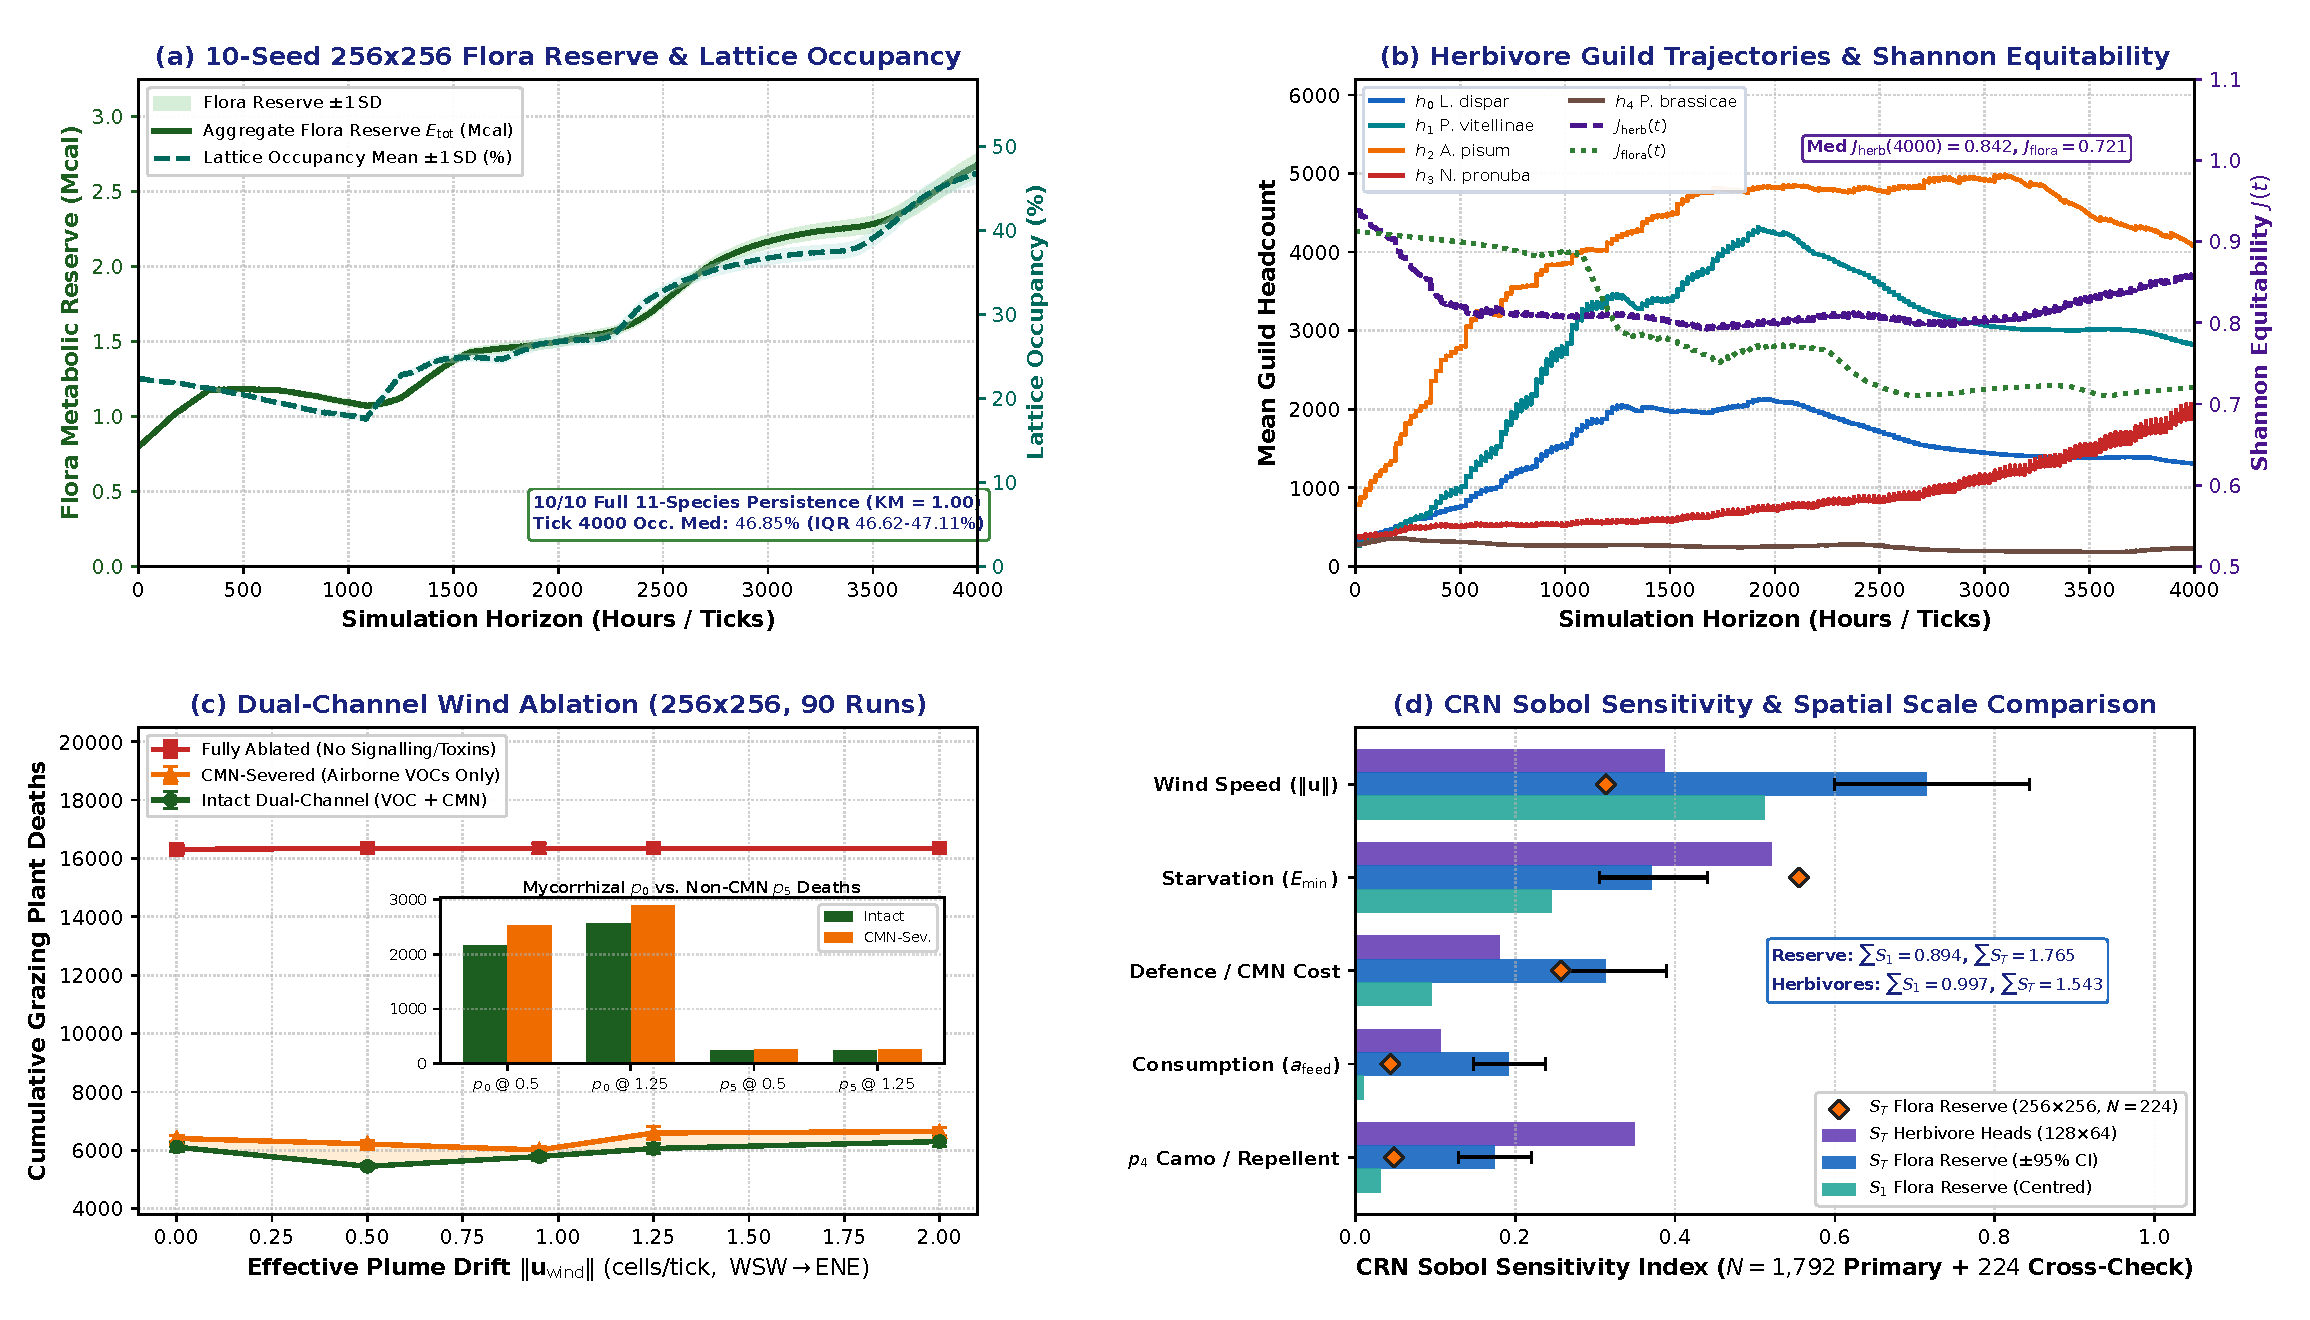
\includegraphics[width=0.92\textwidth]{figures/fig07_multispecies_coexistence.pdf}

  \caption{Empirical Multi-Species Coexistence, Dual-Channel Wind Ablation, and Variance-Based CRN Sobol Sensitivity Analysis on the Central European Ecotone. (a) Ten-seed $256 \times 256$ aggregate flora metabolic reserve ($\text{mean} \pm 1\,\text{SD}$ ribbon, Mcal) and lattice occupancy ($\%$) over $4{,}000$ ticks, reaching $46.85\%$ median terminal occupancy ($Q_{25}\text{--}Q_{75} = 46.62\%\text{--}47.11\%$). (b) Mean herbivore guild trajectories ($h_0$--$h_4$) alongside Shannon--Wiener equitability $J_{\mathrm{flora}}(t)$ and $J_{\mathrm{herb}}(t)$, confirming $10/10$ full $11$-species persistence through tick $4{,}000$. (c) Ninety-run $256 \times 256$ wind and dual-channel ablation across effective plume drift $\|\mathbf{u}_{\mathrm{wind}}\| \in [0.0, 2.0]\,\text{cells/tick}$, contrasting intact, CMN-severed, and fully ablated grazing mortality alongside the mycorrhizal ($p_0$) versus non-mycorrhizal ($p_5$) channel penalty. (d) Converged $128 \times 64$ CRN Sobol sensitivity indices ($N = 1{,}792$ runs, centred Saltelli $S_1$ and Jansen $S_T$ with $95\%$ bootstrap CIs) paired with exploratory $256 \times 256$ cross-check markers ($N = 224$ runs).}
  \label{fig:multispecies_coexistence}
\end{figure*}

Executing a $10$-seed $\times$ $4{,}000$-tick Monte Carlo ensemble (seeds $0\text{--}9$; $1{,}021.7\,\text{s}$ wall-clock across $10$ concurrent workers) evaluates zero-shot spatial scale transfer ($128 \times 64 \to 256 \times 256$) and out-of-sample single-season ($166.7$-day) persistence without retuning (Fig.~\ref{fig:multispecies_coexistence}a--b, Table~\ref{tab:ecotone_ensemble_summary}). Every flora species ($6/6$), every herbivore guild ($5/5$), and joint $11$-species coexistence maintain Kaplan--Meier persistence of $1.00$ ($10/10$ seeds) through tick $4{,}000$. Because the protocol captures one growing season rather than a multi-year stationary climax, directional successional turnover emerges cleanly: aggregate cover roughly doubles from $22.40\%$ to $46.85\%$ median terminal occupancy as cumulative riparian grazing reduces woody \textit{Populus nigra} ($p_0$, $-89\%$) and \textit{Salix purpurea} ($p_1$, $-59\%$) while fast-spreading meadow \textit{Lolium perenne} ($p_3$) expands $3.5\times$, preserving balanced community equitability and bounded oscillatory CVs throughout ticks $1{,}000\text{--}4{,}000$ (Table~\ref{tab:ecotone_ensemble_summary}, Panel~A).

All $12$ defensive pathways remain active during the final $1{,}000$-tick window on every seed, dominated by meadow CMN relays ($s_2$), \textit{Trifolium} phloem withdrawal, and CMN-primed ryegrass/clover toxins ($s_8, s_6$; Table~\ref{tab:ecotone_ensemble_summary}, Panel~B). Detailed instrumentation of \textit{Pieris brassicae} ($h_4$) on a representative trajectory verifies that the nitrile-specifier detoxification gate prevents self-poisoning: $h_4$ incurs zero self-triggered $s_7$ casualties and only $2$ collateral $s_7$ deaths across $11$ exposures (strictly when generalist $h_3$ co-occupies a $p_5$ tile), while $48/50$ toxin casualties occur on non-host meadow toxins ($s_6, s_4$). Consequently, $h_4$ lingers near its low demographic floor not through autotoxicity, but through inter-patch foraging-gap starvation ($23$ starved vs.\ $0$ toxin-killed swarms; $133$ feeding events across $497$ non-repelled daily checks) as larvae navigate the shared chemotactic field between isolated \textit{Brassica} patches ($0.70\% \to 2.80\%$ area).

\begin{table*}[b]
\caption{Ten-Seed $256 \times 256$ Calibrated Ensemble Envelopes at Tick $4{,}000$ and Late-Season ($\Delta_{3\text{k}\to 4\text{k}}$) Cascade Activations.}
\label{tab:ecotone_ensemble_summary}
\vspace{4pt}
\centering
\scriptsize
\setlength{\tabcolsep}{3.0pt}
\begin{tabular*}{\textwidth}{@{\extracolsep{\fill}} l c c @{\hspace{10pt}} l c c c @{}}
\toprule
\multicolumn{7}{@{}l}{\textbf{Panel A: Tick-$4{,}000$ Community Envelopes and Window Temporal CV ($t \in [1{,}000, 4{,}000]$, $10/10$ Full Coexistence)}} \\
\midrule
\textbf{Flora / Metric} & \textbf{Median} & \textbf{IQR ($Q_{25}\text{--}Q_{75}$)} &
\textbf{Herbivore / Metric} & \textbf{Median} & \textbf{IQR ($Q_{25}\text{--}Q_{75}$)} & \textbf{Med CV} \\
\midrule
$p_0$ \textit{Populus nigra}     & $293.0$     & $[215.3, 336.5]$     & $h_0$ \textit{Lymantria dispar}   & $1{,}220.5$ & $[1{,}097.0, 1{,}521.5]$ & $0.193$ \\
$p_1$ \textit{Salix purpurea}    & $690.0$     & $[657.0, 720.0]$     & $h_1$ \textit{Phratora vitellinae}& $2{,}801.0$ & $[2{,}683.8, 3{,}052.3]$ & $0.134$ \\
$p_2$ \textit{Trifolium repens}  & $7{,}351.0$ & $[7{,}054.3, 7{,}508.3]$ & $h_2$ \textit{Acyrthosiphon pisum}& $3{,}861.5$ & $[3{,}687.0, 4{,}681.8]$ & $0.090$ \\
$p_3$ \textit{Lolium perenne}    & $15{,}214.5$& $[15{,}025.3, 15{,}270.3]$& $h_3$ \textit{Noctua pronuba}     & $2{,}061.0$ & $[1{,}600.3, 2{,}249.0]$ & $0.430$ \\
$p_4$ \textit{Tanacetum vulgare} & $5{,}304.0$ & $[5{,}268.8, 5{,}320.0]$ & $h_4$ \textit{Pieris brassicae}   & $142.5$     & $[116.5, 264.8]$         & $0.312$ \\
$p_5$ \textit{Brassica nigra}    & $1{,}831.5$ & $[1{,}806.8, 1{,}844.8]$ & Total Herbivore Heads             & $10{,}421.0$& $[10{,}249.8, 11{,}102.8]$& $---$   \\
Occ.\ ($\%$) / $J_{\text{flora}}$& $46.85$ / $0.7207$ & $[46.62, 47.11]$ / $[0.7165, 0.7241]$ & $J_{\text{herb}}(4000)$ & $0.8418$ & $[0.8324, 0.8512]$ & $---$ \\
\bottomrule
\end{tabular*}

\vspace{3pt}
\begin{tabular*}{\textwidth}{@{\extracolsep{\fill}} l c c @{\hspace{8pt}} l c c @{\hspace{8pt}} l c c @{}}
\toprule
\multicolumn{9}{@{}l}{\textbf{Panel B: Late-Season ($\Delta_{3\text{k}\to 4\text{k}}$) Signalling, Toxin, and Phloem-Withdrawal Activations ($12/12$ Active on $10/10$ Seeds)}} \\
\midrule
\textbf{Channel} & \textbf{Med} & \textbf{IQR} & \textbf{Channel} & \textbf{Med} & \textbf{IQR} & \textbf{Channel} & \textbf{Med} & \textbf{IQR} \\
\midrule
$s_0$ GLV     & $613.0$ & $[522.0, 675.8]$ & $s_4$ Kunitz/Sal.& $354.0$     & $[299.5, 493.0]$   & $s_8$ PPO/Silica & $2{,}092.5$ & $[1{,}690.0, 2{,}423.8]$ \\
$s_1$ Ocimene & $531.0$ & $[455.0, 754.3]$ & $s_5$ Thujone    & $778.0$     & $[694.8, 881.3]$   & Phloem $p_0$     & $269.0$     & $[192.3, 680.5]$ \\
$s_2$ CMN/MeSA& $5{,}901.0$& $[5{,}146.5, 6{,}631.0]$ & $s_6$ HCN & $1{,}435.5$ & $[1{,}273.3, 1{,}718.0]$ & Phloem $p_1$ & $626.0$ & $[574.3, 964.8]$ \\
$s_3$ Benz.\ Cy.& $117.0$ & $[43.3, 238.5]$ & $s_7$ AITC ($h_3$)& $104.0$    & $[57.5, 182.5]$    & Phloem $p_2$     & $5{,}361.0$ & $[3{,}518.8, 7{,}012.3]$ \\
\bottomrule
\end{tabular*}
\end{table*}

% ==============================================================================
\subsection{Diagnostic Evaluation of Analytical Bounds (Propositions~\ref{thm:critical_synthesis_delay} and~\ref{thm:hopf_limit_cycle})}
\label{sec:ecotone_theorem_parity}
% ==============================================================================

We evaluate Propositions~\ref{thm:critical_synthesis_delay} (\eqref{eq:theta_crit_exact}) and~\ref{thm:hopf_limit_cycle} (\eqref{eq:tau_star_exact}) under the runtime Holling Type~II law~\eqref{eq:math_holling_type_ii} across single-cell continuous-grazing sweeps and all $10$ compatible host--herbivore pairs of the calibrated ecotone (Table~\ref{tab:ecotone_theorem_parity}). To project discrete parameters onto the continuous mean-field DDE in Proposition~\ref{thm:hopf_limit_cycle}, effective surrogates map directly from Table~\ref{tab:case_study_configurations} via:
\begin{align}
  a_{\text{eff}, h} &= \frac{a_h}{\max(1, v_h)}, & r_p^{\text{cont}} &= \frac{r_p}{100} \cdot \frac{E_{\mathrm{base}}}{K}, \nonumber \\
  e_{\text{eff}}^{\text{net}} &= \mathrm{clip}\!\left((1 - \delta_m)\,e_{\text{eff}},\, 0,\, 1\right), & m_{\text{herb}} &= E_{\min}^{\text{herb}} \cdot U,
  \label{eq:dde_discrete_conversion}
\end{align}
with $K = E_{\max}$ and $T_h^{\mathrm{stride}}$ taken directly from Panel~B.

Under worst-case continuous hourly grazing ($\Delta t = 1\,\text{h}$, $v = 1$, evaluating Eq.~\eqref{eq:math_holling_type_ii} every tick rather than every $24$ ticks), all single-cell sweeps confirm the closed-form critical boundary $\theta_{\text{crit}}$ cleanly: every latency strictly below $\theta_{\text{crit}}$ preserves foliar survival until toxin deployment, whereas delays above $\theta_{\text{crit}}$ collapse to $E_{\min}$ on the exact predicted tick (Table~\ref{tab:ecotone_theorem_parity}, Panel~A). At outbreak density $N_0 = 16$ (Panel~B), continuous hourly grazing yields $\theta_{\text{crit}} \in [0.3229, 1.1185]\,\text{h}$, breaching every unprimed delay and $9/10$ primed configurations (only \textit{Tanacetum} $\times$ \textit{Noctua} satisfies $\theta_{\mathrm{p}} = 1 < 1.0349\,\text{h}$). Simultaneously, isolated single-tile DDE projections yield unviable caloric fixed points ($E^* \in [0.0081, 0.0713]\,\text{cal} \ll E_{\min}$) and positive leading eigenvalues ($\alpha > 0$) even at $\tau = 0$. Consequently, full-lattice $10/10$ coexistence does not rest on local ODE equilibrium stability, instead emerging from $24$-tick diurnal feeding strides, spatial dispersal, and repellent eviction.

\begin{table*}[b]
\caption{Analytical Bound Verification (Panel~A: Continuous $1\,\mathrm{h}$ Single-Cell Grazing, $v{=}1$) and Outbreak Calibration Diagnostics (Panel~B: $N_0{=}16$ Critical Delay and Lumped DDE Projection via Eq.~\eqref{eq:dde_discrete_conversion}; Unviable $E^* \ll E_{\min}$, $\alpha > 0$ at $\tau{=}0$).}
\label{tab:ecotone_theorem_parity}
\vspace{4pt}
\centering
\scriptsize
\setlength{\tabcolsep}{3.0pt}
\begin{tabularx}{\textwidth}{
  >{\raggedright\hsize=1.00\hsize}X
  >{\centering\hsize=0.55\hsize}X
  >{\centering\hsize=0.70\hsize}X
  >{\raggedright\hsize=1.40\hsize}X
  >{\raggedright\arraybackslash\hsize=1.35\hsize}X
}
\toprule
\multicolumn{5}{@{}l}{\textbf{Panel A: Single-Cell Continuous-Grazing Verification of Proposition~\ref{thm:critical_synthesis_delay} (Eq.~\eqref{eq:theta_crit_exact})}} \\
\midrule
\textbf{Single-Cell Harness ($N_0$)} & \textbf{$\theta_{\text{crit}}$ ($\mathrm{h}$)} & \textbf{Test $\theta$} & \textbf{Surviving ($\theta < \theta_{\text{crit}}$) Outcome} & \textbf{Lethal ($\theta > \theta_{\text{crit}}$) Outcome} \\
\midrule
Reference Baseline ($N_0 = 2$) & $1.5530$ & $\{1, 2, 3, 4\}$ & $\theta = 1$: survives at $10.53\,\mathrm{cal}$ (culled tick $0$) & $\theta \in \{2, 3, 4\}$: plant dies tick $1$ \\
Ecotone $p_3 \times h_3$ ($N_0 = 5$) & $3.5791$ & $\{2, 3, 4, 10\}$ & $\theta \in \{2, 3\}$: survive at $28.41$ / $16.03\,\mathrm{cal}$ & $\theta \in \{4, 10\}$: plant dies tick $3$ \\
Ecotone $p_0 \times h_0$ ($N_0 = 4$) & $1.8372$ & $\{1, 2, 3, 12\}$ & $\theta = 1$: survives at $37.36\,\mathrm{cal}$ (culled tick $0$) & $\theta \in \{2, 3, 12\}$: plant dies tick $1$ \\
\bottomrule
\end{tabularx}

\vspace{3pt}
\setlength{\tabcolsep}{2.5pt}
\begin{tabular*}{\textwidth}{@{\extracolsep{\fill}} l c c c c c c c @{}}
\toprule
\multicolumn{8}{@{}l}{\textbf{Panel B: Compatible Calibrated Ecotone Pairs Under Outbreak Continuous Grazing ($N_0 = 16$) and Zero-Delay DDE Diagnostics}} \\
\midrule
\textbf{Pair} & \textbf{$E_0 / E_{\min}$ ($\mathrm{cal}$)} & \textbf{$a_{\text{eff},h}$ ($\mathrm{str.}^{-1}$)} & \textbf{$T_h^{\mathrm{stride}}$ ($\mathrm{str.}\cdot\mathrm{cal}^{-1}$)} & \textbf{$\theta_{\text{p}} / \theta_{\text{u}}$} & \textbf{$\theta_{\text{crit}}$ ($\mathrm{h}$)} & \textbf{$E^* / N^*$ ($\mathrm{cal} / \mathrm{ind.}$)} & \textbf{$\alpha$ ($\tau = 0$)} \\
\midrule
$p_0 \times h_0$ & $70 / 14$ & $1.6668$ & $0.1140$ & $2 / 12$ & $0.4593$ & $0.0213 / 0.0005$ & $+3.0{\times}10^{-6}$ \\
$p_1 \times h_0$ & $60 / 12$ & $1.6668$ & $0.1140$ & $2 / 12$ & $0.4023$ & $0.0302 / 0.0003$ & $+3.0{\times}10^{-6}$ \\
$p_0 \times h_1$ & $70 / 14$ & $1.1761$ & $0.1726$ & $2 / 12$ & $0.6896$ & $0.0229 / 0.0006$ & $+3.0{\times}10^{-6}$ \\
$p_1 \times h_1$ & $60 / 12$ & $1.1761$ & $0.1726$ & $2 / 12$ & $0.6033$ & $0.0326 / 0.0004$ & $+3.0{\times}10^{-6}$ \\
$p_2 \times h_2$ & $45 / 9$  & $2.6664$ & $0.1268$ & $1 / 8$  & $0.3229$ & $0.0081 / 0.0006$ & $+4.0{\times}10^{-6}$ \\
$p_2 \times h_3$ & $45 / 9$  & $0.5046$ & $0.3342$ & $1 / 8$  & $0.9514$ & $0.0503 / 0.0032$ & $+1.2{\times}10^{-5}$ \\
$p_3 \times h_3$ & $55 / 11$ & $0.5046$ & $0.3342$ & $2 / 10$ & $1.1185$ & $0.0713 / 0.0034$ & $+1.9{\times}10^{-5}$ \\
$p_4 \times h_3$ & $50 / 10$ & $0.5046$ & $0.3342$ & $1 / 3$  & $1.0349$ & $0.0562 / 0.0018$ & $+8.0{\times}10^{-6}$ \\
$p_5 \times h_3$ & $35 / 7$  & $0.5046$ & $0.3342$ & $2 / 8$  & $0.7842$ & $0.0498 / 0.0053$ & $+2.0{\times}10^{-5}$ \\
$p_5 \times h_4$ & $35 / 7$  & $1.3532$ & $0.1633$ & $2 / 8$  & $0.3601$ & $0.0171 / 0.0020$ & $+9.0{\times}10^{-6}$ \\
\bottomrule
\end{tabular*}
\end{table*}

% ==============================================================================
\subsection{Dual-Channel Wind Ablation and Upwind CMN Crossover}
\label{sec:ecotone_ablation}
% ==============================================================================

To separate airborne VOC plumes from subterranean root-link conduits across shifting drift regimes, we executed a $90$-run factorial ablation on the $256 \times 256$ ecotone ($6$ seeds $\times$ $5$ wind speeds $\|\mathbf{u}_{\text{wind}}\| \in [0.0, 2.0]\,\text{cells/tick}$ along WSW$\to$ENE $\times$ $3$ treatments: intact, CMN-severed, and fully ablated; $2{,}500$ ticks; Table~\ref{tab:ecotone_ablation} and Fig.~\ref{fig:multispecies_coexistence}c), paired with a $21$-run deterministic $20$-tick upwind relay test on a $64 \times 64$ seven-plant cardinal chain.

First, removing all signalling and inducible toxins (fully ablated) raises cumulative grazing deaths $2.6\times\text{--}3.0\times$, more than doubles late-horizon herbivore headcounts, and cuts tail flora reserves by roughly $40\%$ (Table~\ref{tab:ecotone_ablation}). Because cleared trigger rules keep every volatile field strictly zero, wind magnitude leaves chemical transport unchanged once signalling is off; seed raycasting uses isotropic sampling under calm air and the normalised unit direction $\mathbf{u}$ along $22.5^\circ$ (Eqs.~\eqref{eq:seed_projection_x}--\eqref{eq:seed_projection_y}) for every positive drift speed, rendering all four positive-drift fully ablated conditions bit-identical on shared seeds (collapsed into the bottom row of Table~\ref{tab:ecotone_ablation}).

Second, severing subterranean CMNs while preserving airborne VOCs increases total grazing mortality across every tested wind speed, peaking at $+14.1\%$ under half-cell drift ($\|\mathbf{u}_{\text{wind}}\| = 0.50\,\text{cells/tick}$, Wilcoxon $p = 0.0312$). Intact grazing deaths attain their global minimum at $0.50\,\text{cells/tick}$, matching the theoretical peak in implicit bilinear numerical diffusion ($\sigma_{\text{num}}^2 = 0.25$, Section~\ref{subsec:operator_splitting}) that widens lateral VOC pre-warming. Disaggregating by guild isolates the statistically consistent CMN-severing penalty squarely on woody mycorrhizal \textit{Populus} ($p_0$, $+10.7\%$ to $+16.7\%$, $p = 0.0312$ across all positive drift speeds), whereas fast-recovering meadow guilds ($p_2 + p_3$) exhibit larger inter-seed variance and the embedded non-mycorrhizal control \textit{Brassica nigra} ($p_5$) displays zero statistically significant sensitivity ($p \ge 0.1562$), confirming specificity to connected root networks. Under the deterministic $20$-tick cardinal relay chain, calm air ($u_x = 0.0$) primes all three upwind and downwind hops symmetrically within ticks $1\text{--}3$. Once $u_x \ge 0.95\,\text{cells/tick}$, airborne-only transport fails completely upwind ($0/3$ hops), whereas intact CMN conduits ($6$ links, $g_{\mathrm{relay}} = 2$) preserve all $3$ upwind priming hops across $u_x \in \{0.95, 1.00, 1.08\}\,\text{cells/tick}$ and $1$ upwind hop at $1.25\,\text{cells/tick}$ before advective washout at $2.00\,\text{cells/tick}$.

\begin{table*}[b]
\caption{Ninety-Run $256 \times 256$ Dual-Channel Wind Ablation Summary ($n=6$ Seeds per Cell, $2{,}500$ Ticks, Mean $\pm$ SE; Paired Wilcoxon $p$ Comparing CMN-Severed vs.\ Intact).}
\label{tab:ecotone_ablation}
\vspace{4pt}
\centering
\scriptsize
\setlength{\tabcolsep}{1.2pt}
\begin{tabular*}{\textwidth}{@{\extracolsep{\fill}} c l c c c c c c c c @{}}
\toprule
\textbf{$\|\mathbf{u}\|$} & \textbf{Treatment} & \textbf{Total $\pm$ SE} & \textbf{Heads} & \textbf{Tail} & \textbf{$J_{\text{f}}$} & \textbf{$J_{\text{h}}$} & \textbf{$p_0 \pm$ SE ($p$)} & \textbf{$p_2{+}p_3 \pm$ SE ($p$)} & \textbf{$p_5 \pm$ SE ($p$)} \\
\midrule
$0.00$ & Intact         & $6{,}108{\pm}146$ & $12{,}728$ & $1.53$ & $.741$ & $.823$ & $2{,}605{\pm}31$ & $1{,}802{\pm}121$ & $231{\pm}9$ \\
$0.00$ & CMN-Sev.       & $6{,}404{\pm}107^{\ast}$ & $13{,}789$ & $1.53$ & $.730$ & $.809$ & $2{,}841{\pm}48$ ($.063$) & $1{,}810{\pm}133$ ($.688$) & $226{\pm}7$ ($.313$) \\
$0.00$ & Ablated        & $16{,}310{\pm}123$& $26{,}952$ & $0.90$ & $.825$ & $.718$ & $3{,}099{\pm}71$ & $10{,}897{\pm}54$ & $581{\pm}18$ \\
\midrule
$0.50$ & Intact         & $5{,}447{\pm}86$  & $11{,}297$ & $1.50$ & $.734$ & $.825$ & $2{,}168{\pm}36$ & $1{,}692{\pm}91$  & $231{\pm}13$ \\
$0.50$ & CMN-Sev.       & $6{,}214{\pm}117^{\ast}$ & $13{,}089$ & $1.50$ & $.728$ & $.827$ & $2{,}529{\pm}33^{\ast}$ ($.031$) & $1{,}994{\pm}108$ ($.063$) & $261{\pm}17$ ($.406$) \\
$0.95$ & Intact         & $5{,}783{\pm}117$ & $11{,}910$ & $1.46$ & $.718$ & $.786$ & $2{,}332{\pm}23$ & $1{,}876{\pm}116$ & $254{\pm}9$ \\
$0.95$ & CMN-Sev.       & $6{,}008{\pm}120$ & $12{,}264$ & $1.48$ & $.710$ & $.831$ & $2{,}644{\pm}36^{\ast}$ ($.031$) & $1{,}721{\pm}105$ ($.313$) & $231{\pm}12$ ($.156$) \\
$1.25$ & Intact         & $6{,}059{\pm}186$ & $12{,}657$ & $1.44$ & $.719$ & $.789$ & $2{,}565{\pm}31$ & $1{,}960{\pm}168$ & $233{\pm}21$ \\
$1.25$ & CMN-Sev.       & $6{,}590{\pm}219$ & $13{,}255$ & $1.47$ & $.711$ & $.817$ & $2{,}893{\pm}28^{\ast}$ ($.031$) & $2{,}028{\pm}191$ ($.688$) & $256{\pm}11$ ($.438$) \\
$2.00$ & Intact         & $6{,}297{\pm}156$ & $13{,}631$ & $1.43$ & $.716$ & $.809$ & $2{,}672{\pm}15$ & $2{,}097{\pm}144$ & $243{\pm}12$ \\
$2.00$ & CMN-Sev.       & $6{,}642{\pm}129$ & $13{,}946$ & $1.46$ & $.708$ & $.817$ & $2{,}957{\pm}44^{\ast}$ ($.031$) & $1{,}994{\pm}140$ ($.313$) & $258{\pm}15$ ($.313$) \\
\midrule
$>0.00^{\dagger}$ & Ablated & $16{,}351{\pm}178$& $27{,}211$ & $0.87$ & $.812$ & $.725$ & $3{,}217{\pm}74$ & $10{,}856{\pm}164$ & $590{\pm}10$ \\
\bottomrule
\multicolumn{10}{@{}p{\textwidth}@{}}{$^{\ast}$Two-sided paired Wilcoxon $p = 0.0312 < 0.05$ ($W = 0.0, n = 6$). Units: $\|\mathbf{u}\|$ ($\mathrm{cells/tick}$), Tail ($\mathrm{Mcal}$). $^{\dagger}$Bit-identical across $\|\mathbf{u}_{\text{wind}}\| \in \{0.50, 0.95, 1.25, 2.00\}\,\mathrm{cells/tick}$ along $22.5^\circ$: inactive chemical triggers leave seed raycasting dependent solely on normalised direction $\mathbf{u}$ (Eqs.~\eqref{eq:seed_projection_x}--\eqref{eq:seed_projection_y}).}
\end{tabular*}
\end{table*}

% ==============================================================================
\subsection{Variance-Based Global Sensitivity Analysis (CRN Sobol GSA)}
\label{sec:ecotone_sobol}
% ==============================================================================

To partition output variance into direct main effects and multi-factor interactions, we apply variance-based Sobol Global Sensitivity Analysis \cite{saltelli2010variance} using a scrambled quasi-random Sobol sequence implemented in SciPy \cite{virtanen2020scipy}. For a scalar output $Y = f(\mathbf{X})$ over $k$ independent inputs $\mathbf{X} = (X_1, \dots, X_k)$, the orthogonal Hoeffding--Sobol decomposition defines first-order ($S_i$) and total-order ($S_{T_i}$) indices:
\begin{align}
  S_i &= \frac{V_{X_i}\!\left(\mathbb{E}_{\mathbf{X}_{\sim i}}[Y \mid X_i]\right)}{V(Y)}, \nonumber \\
  S_{T_i} &= \frac{\mathbb{E}_{\mathbf{X}_{\sim i}}\!\left[V_{X_i}(Y \mid \mathbf{X}_{\sim i})\right]}{V(Y)} = 1 - \frac{V_{\mathbf{X}_{\sim i}}\!\left(\mathbb{E}_{X_i}[Y \mid \mathbf{X}_{\sim i}]\right)}{V(Y)},
  \label{eq:sobol_def}
\end{align}
evaluated via a Saltelli radial design ($N = n_{\text{base}}(k + 2)$ runs) over sample matrices $\mathbf{A}, \mathbf{B} \in \mathbb{R}^{n_{\text{base}} \times k}$ and hybrid blocks $\mathbf{A}_{\mathbf{B}}^{(i)}$ \cite{saltelli2010variance}. Holding the stochastic seed fixed across every design row (Common Random Numbers, CRN) eliminates between-seed Monte Carlo variance. Because mean flora reserve exhibits a high mean-to-standard-deviation ratio ($\mu / \sigma \approx 11.9$), subtracting the pooled baseline mean $\bar{y}$ of $\mathbf{A} \cup \mathbf{B}$ alongside the Jansen estimator \cite{jansen1999analysis} stabilises finite-sample estimation:
\begin{align}
  \hat{S}_i &= \frac{\frac{1}{n_{\mathrm{base}}}\sum_{j=1}^{n_{\mathrm{base}}} \left(y_{\mathbf{B},j} - \bar{y}\right)\left(y_{\mathbf{A}_{\mathbf{B}}^{(i)},j} - y_{\mathbf{A},j}\right)}{\widehat{V}_{\mathbf{A}\cup\mathbf{B}}(Y)}, \nonumber \\
  \hat{S}_{T_i} &= \frac{\frac{1}{2\,n_{\mathrm{base}}}\sum_{j=1}^{n_{\mathrm{base}}} \left(y_{\mathbf{A},j} - y_{\mathbf{A}_{\mathbf{B}}^{(i)},j}\right)^2}{\widehat{V}_{\mathbf{A}\cup\mathbf{B}}(Y)},
  \label{eq:sobol_estimators}
\end{align}
using unbiased sample variance over $\mathbf{A} \cup \mathbf{B}$ and $500$ bootstrap resamples for $95\%$ confidence intervals.

We jointly sampled $k = 5$ biophysical multipliers across per-stride consumption rate ($\kappa_a$), herbivore starvation threshold ($\kappa_{E_{\min}}$), combined defence and CMN upkeep ($\kappa_{\mathrm{cost}}$), effective plume drift ($\|\mathbf{u}_{\text{wind}}\|$), and $p_4$ olfactory strength ($s_{p_4}$, setting $\Phi_{\text{camo}} = 1 - 0.75 s_{p_4}$ and $s_5$ eviction duration $\max(1, \mathrm{round}(8 s_{p_4}))$). The primary $128 \times 64$ GSA executed $n_{\text{base}} = 256$ ($N = 1{,}792$ runs, $1{,}500$ ticks, $6{,}991.5\,\text{s}$), paired with an exploratory $256 \times 256$ cross-check ($n_{\text{base}} = 32$, $N = 224$ runs, $1{,}000$ ticks, $3{,}712.7\,\text{s}$).

Across all $15$ factor--output pairs of the converged $128 \times 64$ suite (Table~\ref{tab:ecotone_sobol}, Fig.~\ref{fig:multispecies_coexistence}d), $S_1 \le S_T$ holds strictly throughout with total-order indices summing cleanly to $\sum S_T \in [1.543, 1.938]$ ($\sum S_1 \in [0.838, 0.997]$; the lone small negative Saltelli estimate $S_1 = -0.042$ for $\kappa_{\mathrm{cost}}$ on $J_{\text{flora}}$ reflects finite-sample estimator noise around a near-zero main effect). Plume drift $\|\mathbf{u}_{\text{wind}}\|$ dominates both aggregate vegetation reserve and terminal flora equitability, whereas the herbivore starvation threshold $\kappa_{E_{\min}}$ governs terminal herbivore headcounts; $p_4$ olfactory shielding and defence/CMN costs contribute predominantly through multi-factor interactions ($S_T \gg S_1$). In addition, consumption-rate scaling $\kappa_a$ exhibits negligible direct main effects ($S_1 \le 0.027$) across all outputs and both lattice scales, confirming the kinetic mechanism in Eq.~\eqref{eq:math_holling_type_ii}: because diurnal calibrated parameters operate near the Holling Type~II saturation ceiling $1/T_h^{\mathrm{stride}}$ ($a_{\mathrm{eff}} T_h^{\mathrm{stride}} E \approx 9.3 \gg 1$ on meadow clover and ryegrass), perturbations in attack rate minimally alter per-event intake compared against advective plume geometry and metabolic starvation thresholds. Despite finite-sample Saltelli noise at $n_{\text{base}} = 32$ ($S_1 \in [-0.111, +0.593]$, one sample exceedance $S_1 = +0.268 > S_T$ for $\kappa_{\mathrm{cost}}$ on reserve), the $256 \times 256$ cross-check preserves the identical dominance hierarchy ($\kappa_{E_{\min}}$ and $\|\mathbf{u}_{\text{wind}}\|$ leading; $\kappa_a$ negligible).

\begin{table*}[b]
\caption{CRN Sobol Sensitivity Indices: Primary Converged $128 \times 64$ Design ($n_{\mathrm{base}}{=}256$, $N{=}1{,}792$, $1{,}500$ Ticks; $S_1$ Centred Saltelli and $S_T$ Jansen with $95\%$ Bootstrap CIs) Alongside Exploratory $256 \times 256$ Cross-Check ($n_{\mathrm{base}}{=}32$, $N{=}224$, $1{,}000$ Ticks).}
\label{tab:ecotone_sobol}
\vspace{4pt}
\centering
\scriptsize
\setlength{\tabcolsep}{1.8pt}
\begin{tabular*}{\textwidth}{@{\extracolsep{\fill}} l c c c @{\hspace{6pt}} c c c @{\hspace{6pt}} c c c @{}}
\toprule
\textbf{Factor (Range)} &
\multicolumn{3}{c}{\textbf{Mean Flora Reserve}} &
\multicolumn{3}{c}{\textbf{Terminal $J_{\text{flora}}$}} &
\multicolumn{3}{c}{\textbf{Terminal Herbivore Heads}} \\
\cmidrule(lr){2-4} \cmidrule(lr){5-7} \cmidrule(lr){8-10}
& \textbf{$S_1$} & \textbf{$S_T$ [$95\%$ CI]} & \textbf{$S_T^{(256)}$} &
  \textbf{$S_1$} & \textbf{$S_T$ [$95\%$ CI]} & \textbf{$S_T^{(256)}$} &
  \textbf{$S_1$} & \textbf{$S_T$ [$95\%$ CI]} & \textbf{$S_T^{(256)}$} \\
\midrule
Intake $\kappa_a$ ($[0.8, 1.4]$) &
$+0.011$ & $0.192\,[0.148, 0.238]$ & $0.044$ &
$+0.027$ & $0.264\,[0.213, 0.326]$ & $0.128$ &
$+0.005$ & $0.106\,[0.087, 0.132]$ & $0.033$ \\
Starv.\ $\kappa_{E_{\min}}$ ($[0.7, 1.3]$) &
$+0.245$ & $0.371\,[0.305, 0.441]$ & $0.555$ &
$+0.223$ & $0.403\,[0.331, 0.483]$ & $0.502$ &
$+0.440$ & $0.521\,[0.437, 0.614]$ & $0.674$ \\
Cost $\kappa_{\mathrm{cost}}$ ($[0.5, 1.5]$) &
$+0.095$ & $0.313\,[0.253, 0.390]$ & $0.257$ &
$-0.042$ & $0.245\,[0.198, 0.299]$ & $0.171$ &
$+0.088$ & $0.180\,[0.141, 0.233]$ & $0.098$ \\
Drift $\|\mathbf{u}_{\text{wind}}\|$ ($[0, 2]\,\mathrm{c/t}$) &
$+0.512$ & $0.715\,[0.599, 0.844]$ & $0.314$ &
$+0.567$ & $0.731\,[0.624, 0.856]$ & $0.561$ &
$+0.259$ & $0.387\,[0.315, 0.464]$ & $0.176$ \\
Camo $s_{p_4}$ ($[0.2, 1.0]$) &
$+0.031$ & $0.174\,[0.129, 0.220]$ & $0.048$ &
$+0.063$ & $0.296\,[0.235, 0.369]$ & $0.109$ &
$+0.206$ & $0.349\,[0.283, 0.429]$ & $0.063$ \\
\midrule
\textbf{Index Sums ($\sum S_1 / \sum S_T$)} &
$0.894$ & $1.765$ & $1.218$ &
$0.838$ & $1.938$ & $1.470$ &
$0.997$ & $1.543$ & $1.044$ \\
\bottomrule
\multicolumn{10}{@{}p{\textwidth}@{}}{$128 \times 64$ output distributions (mean $\pm$ SD): flora reserve $145{,}228 \pm 12{,}240\,\mathrm{cal}$, $J_{\text{flora}} = 0.768 \pm 0.052$, herbivore heads $2{,}200.5 \pm 742.8$. Exploratory $256 \times 256$ distributions: reserve $1{,}150{,}485 \pm 51{,}017\,\mathrm{cal}$, $J_{\text{flora}} = 0.884 \pm 0.015$, heads $10{,}530.2 \pm 2{,}994.4$. Units: $\mathrm{c/t} \equiv \mathrm{cells/tick}$.}
\end{tabular*}
\end{table*}
